\documentclass[conference]{IEEEtran}
\IEEEoverridecommandlockouts
% The preceding line is only needed to identify funding in the first footnote. If that is unneeded, please comment it out.
%Template version as of 6/27/2024

\usepackage{cite}
\usepackage{float}
\usepackage{amsmath,amssymb,amsfonts}
\usepackage{algorithmic}
\usepackage{graphicx}
\usepackage{textcomp}
\usepackage{xcolor}
\usepackage{booktabs}
\usepackage{tabularx}
\usepackage{subcaption}
\usepackage[T1]{fontenc}
\usepackage{threeparttable}
\usepackage{hyperref}
\usepackage{siunitx}


\def\BibTeX{{\rm B\kern-.05em{\sc i\kern-.025em b}\kern-.08em
    T\kern-.1667em\lower.7ex\hbox{E}\kern-.125emX}}
\begin{document}

\title{Design and Evaluation of  Two Spherical Systems for 3D Mapping*\\

%\thanks{Identify applicable funding agency here. If none, delete this.}
}

\author{\IEEEauthorblockN{Marawan Khalil, Fabian Arzberger, and Andreas Nüchter}
\IEEEauthorblockA{\textit{Computer Science XVII – Robotics} \\
\textit{Julius-Maximilians-University}\\
Würzburg, Germany \\
marawan.khalil@stud-mail.uni-wuerzburg.de, \{fabian.arzberger, andreas.nuechter\}@uni-wuerzburg.de}
}

\maketitle

\begin{abstract}
Spherical robots offer unique advantages for mapping applications in hazardous or confined environments, thanks to their protective shells and omnidirectional mobility. 
This work presents two complementary spherical mapping systems: a lightweight, non-actuated design and an actuated variant featuring internal pendulum-driven locomotion. 
Both systems are equipped with a Livox Mid-360 solid-state LiDAR sensor and run Lidar-Inertial Odometry (LIO) algorithms on resource-constrained hardware. 
We asses the mapping accuracy of these systems by comparing the resulting 3D point-clouds from the LIO algorithms to a ground truth map.
The results indicate that the performance of state-of-the-art LIO algorithms deteriorates due to the high dynamic movement introduced by the spherical locomotion, leading to globally inconsistent maps and sometimes unrecoverable drift.
%A comparative evaluation highlights distinct performance characteristics: the non-actuated sphere achieves higher mapping accuracy, while the actuated system provides denser point clouds and shows potential for autonomous navigation. 
%These results lay the groundwork for deploying spherical robots in challenging environments such as underground infrastructure or planetary surfaces, where traditional robotic platforms often face operational constraints.
\end{abstract}

\begin{IEEEkeywords}
Spherical robots, Mobile mapping, Actuation Mechanisms, LiDAR, SLAM.
\end{IEEEkeywords}

\section{Introduction}
In recent decades, robotics has evolved from a niche discipline into a transformative technology impacting a wide range of industries, including manufacturing, healthcare, space exploration, and personal assistance. 
Among the diverse types of robotic systems, spherical robots have recently begun to attract increased attention from researchers. These robots represent a relatively unconventional design compared to more familiar, rotation-restricted systems such as UAVs, handheld devices, and wheeled vehicles. 
Unlike traditional wheeled or legged robots, spherical robots offer several key advantages, including omnidirectional movement, enhanced maneuverability in unpredictable environments, and improved protection for internal components. 
These features make them well-suited for a variety of applications such as surveillance, inspection, environmental monitoring in hazardous conditions, and search-and-rescue operations. 
Their spherical design enables them to access environments that are difficult or impossible for other robotic systems to navigate, such as steep tunnels, underground mines, narrow passageways, and other confined or dangerous spaces.
The sealed outer shell of a spherical robot provides full protection against dust, hazardous chemicals, liquids, and external impacts. 
Recent research has focused on developing more robust motion mechanisms \cite{roboball,novelsphere,pendulum_sphere} and incorporating technologies like LiDAR for 3D mapping, further expanding their capabilities in complex and unpredictable environments\cite{Kalman_filter_sphere,DAEDALUS,sphere_Fabi_1}.

This research focuses on the development and evaluation of two custom-built spherical robots (see~\ref{fig:twospheres}) equipped with LiDAR-based SLAM systems. 
Both systems integrate Fast-LIO2\cite{fastlio2}, Fast-LIVO2\cite{fastlivo2}, and DLIO\cite{dlio}, which are state-of-the-art LiDAR-inertial odometry algorithms.
In the next section, we review recent advancements in spherical robot design and the latest developments in SLAM for spherical platforms, with a particular emphasis on LiDAR-inertial methods. 
In \ref{sec:hardwaredesing}, we give a description of the hardware implementation of the two spherical robots. 
Subsequently, we describe the software integration, as well as the motion control mechanisms used for the actuated sphere. 
Finally, we provide a comprehensive evaluation of the mapping accuracy by comparing the maps of the proposed systems with a ground truth map available from high precise terrestrial laser scanning (TLS). 

\begin{figure}[t]
\centerline{\includegraphics[width=0.7\columnwidth]{pics/two_spheres.jpg}}
\caption{(Left:) 20cm$\varnothing$ Actuated Sphere. (Right:) 16cm$\varnothing$ Non-actuated Sphere.}
\vspace{-15pt}
\label{fig:twospheres}
\end{figure}
\section{State of the Art}

\subsection{Spherical SLAM}\label{AA}

Spherical Simultaneous Localization and Mapping (SLAM) is an emerging area within mobile robotics, offering promising solutions for robust mapping in constrained or hazardous environments. 
Unlike traditional platforms, spherical robots encapsulate their sensors within a protective shell and rely on rolling locomotion. 
This unique configuration introduces both opportunities and significant challenges for SLAM algorithms. 
One of the earliest spherical SLAM prototypes was L.U.N.A. \cite{luna} , which employed a 2D LiDAR and IMU inside a rolling spherical shell. 
The design validated the feasibility of spherical SLAM. 
It also featured actuation through internal flywheels, using an IBCOAM (Impulse by Conservation of Angular Momentum) mechanism.
A major milestone in this field was the DAEDALUS project \cite{DAEDALUS}, funded by the European Space Agency, which proposed a fully enclosed spherical robot for the autonomous exploration of lunar lava tubes. 
The robot is suggested to be equipped with LiDAR and internal actuators, and its design focused on resilience to lunar regolith and harsh environmental conditions.
A core challenge in spherical SLAM is the aggressive and non-centered rotation induced by rolling locomotion. 
These motions produce high angular velocities and dynamic behavior across all principal axes. 
This significantly degrades pose estimation accuracy and leads to error accumulation in the map. 
This problem is further compounded by the absence of magnetometer usage—often intentionally excluded due to the unreliability of magnetic field data in planetary environments, which leads to uncorrected yaw drift in IMU-based odometry, especially during prolonged navigation.
To address these issues, Arzberger et al. \cite{Kalman_filter_sphere,sphere_Fabi_1,DeltaFilter} introduced specialized filtering techniques for spherical systems. 
Their Delta Filter is a lightweight, real-time, multi-trajectory pose estimation method that fuses unreliable trajectories, such as those from IMUs and stereo visual-inertial odometry (VIO), into a more robust estimate, without requiring explicit sensor uncertainty modeling. 
The filter operates on pose changes ("deltas"), uses a probabilistic weighting scheme for translation estimation, and applies rotational interpolation via spherical linear interpolation (Slerp). 
A follow-up Kalman Filter design extended this approach by incorporating covariance-aware models, enhancing pose estimation accuracy during rapid and complex motion.
% Despite these advances, most current spherical SLAM systems still lack precise onboard actuation for controlled repositioning beyond rolling, limiting their effectiveness in tightly constrained environments. 
While recent studies (e.g. \cite{Kalman_filter_sphere}) have compared their results with state-of-the-art SLAM systems such as DLIO\cite{dlio} and FAST-LIO2\cite{fastlio2}, the field continues to evolve rapidly. 
More recent SLAM algorithms (e.g., FAST-LIVO2\cite{fastlivo2}), advanced LiDARs like the MID-360 and RoboSense Airy, and modern microprocessors such as the Raspberry Pi 5 with PCIe support and Gigabit Ethernet are pushing the boundaries of what is possible. 
In this context, we introduce our first prototype, the Non-actuated Sphere, which leverages the processing power of the Raspberry Pi 5 16GB RAM model. 
This design enables real-time SLAM on a compact spherical platform,  offering improved power efficiency, extended battery life, and reduced overall system cost.
\subsection{Spherical locomotion}

\label{sec:state-of-the-art}

Spherical locomotion has attracted significant research interest in recent years, driven by the pursuit of optimal mobility mechanisms. 
Although spherical robots may appear mechanically simple, a wide variety of locomotion strategies have been developed—and continue to emerge—requiring sophisticated control systems to manage the complex dynamics of rolling locomotion and internal mass distribution.
One of the most well-known approaches is the Internal Driving Unit (IDU), or differential drive, used in commercial robots like the Sphero Bolt+ and BB-8. 
Akella et al.\cite{Sphero} analyzed BB-8’s internal wheel-driven system and demonstrated that effective control could be achieved using only two actuators. 
However, they highlighted a key limitation: the robot’s geometry prevents controlled sliding and reduces effectiveness on inclined or uneven terrain.
In contrast, Zevering et al.~\cite{luna} introduced L.U.N.A., a spherical robot designed for autonomous 3D mapping in lunar caves. 
Rather than using wheels or rods, L.U.N.A. relies on internal flywheels to generate motion via the IBCOAM method. 
This approach enables a compact form factor and protects internal electronics, providing advantages particularly well suited to harsh and remote terrain. 
The robot demonstrated reliable motion on soft surfaces such as sand and rubber. 
However, limitations remain, including vibrational instability caused by unbalanced flywheels, reduced performance on inclined low-friction surfaces, and pose estimation errors due to unsynchronized sensor data.
In a following study by Zevering et al.~\cite{rod_sphere} proposed a rod-driven spherical robot, also targeting lunar cave exploration. 
This design uses external linear actuators to push against the environment to induce motion. 
While it improves adaptability to rugged terrain and sharp obstacles, it introduces new challenges, such as oscillatory behavior from fixed-speed actuators, limited effectiveness on slopes, and the need for higher-power actuation when traversing dusty or soft ground.
Beyond differential and flywheel-based designs, several researchers have explored pendulum-driven locomotion due to its mechanical simplicity, energy efficiency, and natural stability. 
Oevermann et al.~\cite{roboball}, Ren et al.~\cite{novelsphere}, and  Kolbari et al.~\cite{pendulum_sphere} developed spherical robots that use an internal heavy pendulum as the primary driving mechanism. 
While their configurations differ in terms of shell design and target applications, they share a common reliance on pendulum-based locomotion and have demonstrated robust movement across a variety of terrains.
A notable example is RoboBall~\cite{roboball}, which features a novel soft pressurized shell and a two-degree-of-freedom internal pendulum. 
This robot successfully navigates gravel, grass, steep inclines, and even floats and maneuvers on water. 
However, the deformable shell introduces complex dynamic behaviors. 
These were addressed using a Linear Quadratic Regulator (LQR) for steering and a model-based proportional controller for driving. 
In contrast, \cite{novelsphere} and \cite{pendulum_sphere} adopted PID-based stabilization strategies to enhance motion control and responsiveness. 
RoboBall’s experiments further revealed that internal pressure and shell deformation significantly affect dynamic behavior—especially due to the presence of a ``dead zone'' where balance control becomes unstable during motion.
Taken together, these pendulum-based locomotion strategies highlight the value of combining mechanical simplicity with robust control to enable adaptive movement in unpredictable environments. 
While a variety of innovative locomotion methods have been proposed for spherical robots, including flywheel-, rod-, and pendulum-driven systems, few have been evaluated in conjunction with advanced LiDAR-inertial odometry algorithms under real-world motion dynamics.
This paper addresses this gap by introducing our second prototype, a pendulum-driven spherical robot designed to achieve both robust locomotion and accurate, real-time mapping performance within the constraints of a compact platform.

\section{Hardware and Design}
\label{sec:hardwaredesing}

This section describes the hardware design and structural implementation of two spherical robots developed for 3D mapping: the Non-actuated Sphere and the Actuated Sphere.
 \subsection{Non-Actuated Sphere}

The non-actuated sphere was modeled using CAD software, drawing inspiration from~\cite{Kalman_filter_sphere} design. 
Its structure consists of two flat discs stacked vertically and secured with pillar screws, maintaining a gap of approximately \SI{28}{\milli\meter} between them. 
%The diameter of the discs was calculated using the Pythagorean theorem to ensure proper spacing and balance.
To enhance structural integrity and safety, fillets were applied to the edges of the discs. 
Each disc has a uniform thickness of \SI{3}{\milli\meter}.
Two fabrication methods were used to produce the discs: 3D printing with PLA and laser cutting with acrylic. 
%Both materials demonstrated sufficient durability during initial testing.
Table~\ref{tab:hardware_components_non_actuated} summarizes the components used in the non-actuated sphere and its location within the sphere.

\begin{table}
\centering
\caption{Hardware Components and Their Placement Inside the Sphere}
\label{tab:hardware_components_non_actuated}
\begin{tabularx}{\linewidth}{@{}l X@{}}
\toprule
\textbf{Layer} & \textbf{Components} \\
\midrule
Top    & Livox Mid-360 LiDAR, BNO-085 IMU \\
Middle & Raspberry Pi 5 (16 GB, 256 GB SSD, cooling fan) \\
       & 2200 mAh 3S LiPo battery \\
Bottom & Voltage regulators \\
\bottomrule
\end{tabularx}
\vspace{-1em}
\end{table}

\begin{figure}
\centering
\begin{subfigure}{0.4\columnwidth}
    \centering
    \includegraphics[width=\textwidth]{pics/Non_actuated_Sphere_CAD.png}
    \caption{3D CAD Model}
    \label{fig:cad-model}
\end{subfigure}
\hfill
\begin{subfigure}{0.4\columnwidth}
    \centering
    \includegraphics[width=\textwidth]{pics/image.png}
    \caption{Simplified 2D Model}
    \label{fig:2d-model}
\end{subfigure}
\caption{Different views of the Non-actuated sphere.}
\vspace{-10pt}
\label{fig:cad-design1}
\end{figure}

The Livox Mid-360 is connected to the Raspberry Pi via Ethernet, while the BNO-085 IMU communicates using the I2C interface. 
The sphere is designed to be lightweight, with a total weight of approximately \SI{1}{\kilo\gram}, including the battery and all internal components. 
The sphere's diameter is \SI{16}{\centi\meter}. 
It is designed to be rolled manually by foot or hand.
To ensure stable and predictable rotation, metal weights were placed within the sphere to align its center of mass with its geometric center. 
A 3D CAD model of the assembled structure is shown in Fig.~\ref{fig:cad-design1}.



\subsection{Actuated Sphere}

The actuated sphere was designed using CAD software, with Fig.~\ref{fig:cad-design2} illustrating the final structure. 
As described in Section~\ref{sec:state-of-the-art}, the design was inspired by the pendulum-driven locomotion mechanisms presented in studies~\cite{roboball, novelsphere}.
Unlike the non-actuated version, this sphere features an internal actuation system. 
At its core, a Waveshare Smart Continuous Servo (model ST3215) is mounted to control forward and backward motion by dynamically shifting the internal center of mass in the direction of travel. 
A second PWM-controlled servo enables left and right movement via pendulum displacement along the lateral axis.
The structural components were fabricated using PLA filament and 3D-printed in three separate pieces, which are then assembled into the complete sphere.
The system dynamics as shown in Fig.~\ref{fig:2d-model2} involve key parameters including the robot’s horizontal position \( x \), the spinning angle of the shell \( \phi \), the swinging angle of the counter-weight mass \( \alpha \), and the input torque of the primary motor \( \tau \). 
Associated physical properties include the shell mass \( m_1 \), inner driver mass \( m_2 \), counter-weight mass \( m_3 \), gravitational acceleration \( g \), and the length of the connecting rod \( l \). 
%All of this is taken into consideration when designing the sphere and its control system.
The internal hardware components are organized according to their position within the sphere, as detailed in Table~\ref{tab:hardware_components_actuated}.

\begin{figure}
\begin{subfigure}{0.4\columnwidth}
    \centering
    \includegraphics[width=\textwidth]{pics/Actuated_sphere.png}
    \caption{3D CAD model}
    \label{fig:cad-design2}
\end{subfigure}
\hfill
\begin{subfigure}{0.4\columnwidth}
    \centering
    \includegraphics[width=\textwidth]{pics/planer_model.png}
    \caption{Simplified 2D Model\cite{Sphere_2D}}
    \label{fig:2d-model2}
\end{subfigure}
\caption{Different views of the Actuated sphere.}
\label{fig:cad-design2}
\end{figure}

\begin{figure*}
    \centering
    \includegraphics[width=1\linewidth]{pics/Khonsu.pdf} 
    \caption{State chart of the Sphere System showing the control and mapping subsystems.}
    \label{fig:sphere_system}
\end{figure*}

\begin{table}
\centering
\caption{Hardware Components and Their Placement Inside the Sphere}
\label{tab:hardware_components_actuated}
\begin{tabularx}{\linewidth}{@{}l X@{}}
\toprule
\textbf{Position} & \textbf{Components} \\
\midrule
Center & Waveshare Smart Continuous Servo (model ST3215) \\
       & Forward/backward actuation \\
       & PWM Servo – left/right pendulum control \\
Rear   & 2200 mAh 3S LiPo battery \\
       & 5V 5A voltage regulator (for Raspberry Pi 5) \\
       & 6V UBEC (for servo motors) \\
Pendulum Module & 12V 20A voltage regulator – powers the entire system; positioned near the shell for stability \\
Front  & Raspberry Pi 5 (16 GB model) \\
Top    & Livox Mid-360 LiDAR \\
       & Pi Camera V3 (12 MP) \\
\bottomrule
\end{tabularx}
\end{table}

\section{Software and Control System}

As shown in the system state diagram Fig.~\ref{fig:sphere_system}, both the actuated and non-actuated spheres follow the same state transitions, with the exception of the control subsystem, which is unique to the actuated variant. 
All software components are deployed on Ubuntu 24.04.2 LTS ARM and ROS 2 Jazzy.

\subsection{Mapping System}

Both spheres incorporate a real-time mapping system. 
The following LiDAR-Inertial Odometry (LIO) frameworks were evaluated and integrated:

\begin{itemize}
    \item \textbf{FAST-LIO2}
    \item \textbf{DLIO}
    \item \textbf{FAST-LIVO2} (used in LIO-only mode)
\end{itemize}

Some packages needed modification to meet the constraints and processing capabilities of the Raspberry Pi 5 and ROS2 Jazzy.
The source code is available in our GitHub repository~\cite{githubsphere}.
All mapping computations are performed onboard in real-time.
%Resulting maps are stored in ros bag format for later evaluation and comparison against ground truth data.

\subsection{Actuator System (Actuated Sphere Only)}

The actuated sphere features an internal movement control system, operated using a  Logitech F710 controller. 
The controller's two joysticks are mapped to distinct control tasks:

\begin{itemize}
    \item \textbf{Servo control:} One joystick provides input to the continuous rotation servo. 
    These inputs are scaled and passed through a discrete Proportional-Integral-Derivative (PID) controller to regulate pitch by minimizing the error between a desired target angle and the current angle measured by the IMU.
    \item \textbf{Mass shifting:} The second joystick adjusts the angle of an internal weight to shift the center of mass left or right, enabling directional control of the sphere's rolling behavior.
\end{itemize}

% \begin{equation}
% u[k] = K_p \cdot e[k] + K_i \cdot \sum_{i=0}^{k} e[i] \cdot \Delta t + K_d \cdot \frac{e[k] - e[k-1]}{\Delta t} \label{eq:pid_control}
% \end{equation}

% where \( u[k] \) is the servo motor command at time step \( k \), \( e[k] \) is the pitch error defined as the difference between the target angle \( \theta_{\text{target}} \) and the current angle \( \theta_{\text{current}} \), and \( K_p \), \( K_i \), \( K_d \) are the proportional, integral, and derivative gains, respectively. The controller runs at a fixed sampling interval \( \Delta t \) and includes a small deadband around the setpoint to reduce oscillations. Within this deadband, the integral term is reset to prevent windup. Additionally, manual control inputs can be superimposed onto the PID output, enabling user intervention without disrupting balance. The resulting command is then limited to a predefined range before being sent to the servo motor, which also considers real-time motor speed and IMU feedback to maintain stable velocity and orientation.

This control strategy allows for fine-grained movement and stabilization, combining feedback-based servo control with physical mass displacement for maneuvering.


\section{Evaluation and Results}
In this section, we present the evaluation and results of both spherical robots in terms of their mapping accuracy and stability.
All experiments were conducted in a controlled indoor environment within the Computer Science building at the University of Würzburg.

\subsection{Evaluation Setup}
The evaluation consisted of mapping selected indoor areas—specifically, a corridor, a hall, and the upper floor—using both the non-actuated and actuated spherical robots. 
For the non-actuated sphere, the robot was manually moved by hand and by foot. 
Each mapping run used one of three SLAM algorithms: Fast-LIO2, DLIO, and Fast-LIVO2 (LIO mode). 
The experiment was repeated three times—once for each algorithm—under the same environmental conditions. 
The same procedure was carried out with the actuated sphere, with the key difference being that it was moved using a controller rather than manually. 
Again, each of the three SLAM algorithms was executed along similar paths within the same locations. 
We used 3DTK~\cite{3dtk} to process the resulting point clouds, which were evaluated by comparing them against ground-truth data obtained using a Riegl VZ-400 terrestrial laser scanner (TLS) as shown in Fig.~\ref{fig:riegl}.

\begin{figure}[t]
\centering
\begin{subfigure}{0.48\columnwidth}
        \centering
        \includegraphics[width=\textwidth]{pics/riegl.jpg}
        \caption{Riegl VZ-400 with both spheres.}
        \label{fig:riegl}\end{subfigure}
\hfill
\begin{subfigure}{0.48\columnwidth}
        \centering
        \includegraphics[width=\textwidth]{pics/sphere_on_the_move.jpeg}
        \caption{Point clouds from the Riegl VZ-400.}
        \label{fig:sphere_on_the_move}
\end{subfigure}
\caption{Evaluation Setup, showing the Riegl VZ-400 TLS and the spheres in action. A video where both spheres are moving can be found at \url{https://youtu.be/1b0d2g3k4e8}.}

\end{figure}

\begin{figure}[t]
\centering
\begin{subfigure}{0.48\columnwidth}
        \centering
        \includegraphics[width=\textwidth]{pics/eagle_view/riegl_top.png}
        \caption{Resulted Riegl Map}
        \label{fig:riegl_top}\end{subfigure}
\hfill
\begin{subfigure}{0.48\columnwidth}
        \centering
        \includegraphics[width=\textwidth]{pics/eagle_view/act_livo_to.png}
        \caption{Actuated Fast-LIVO2}
        \label{fig:act_livo_top}
\end{subfigure}

\begin{subfigure}{0.48\columnwidth}
        \centering
        \includegraphics[width=\textwidth]{pics/eagle_view/act_lio_top.png}
        \caption{Actuated Fast-LIO2}
        \label{fig:act_fast_lio_top}\end{subfigure}
\hfill
\begin{subfigure}{0.48\columnwidth}
        \centering
        \includegraphics[width=\textwidth]{pics/eagle_view/non_lio_top.png}
        \caption{Non-actuated Fast-LIO2}
        \label{fig:non_act_fast_lio_top}
\end{subfigure}

\caption{Cross Section of resulted maps(Height gradient).}

\end{figure}

\subsubsection{Point cloud error}
The point cloud error represents the root of the mean squared point-to-point errors (RMSE).
\begin{equation}
    RMSE = \sqrt{\frac{1}{N} \sum_{i=1}^{N} |p_i - q_i|^2}
\end{equation}
where \( p_i \) and \( q_i \) are the corresponding points in the model and data point clouds, and \( N\) is the number of corresponding points. 
The RMSE is a measure of the average distance between the points in the two point clouds, providing an indication of the mapping accuracy.
% \subsubsection{Steady-state error}

% The steady-state error is defined as the difference between the desired and actual position of the sphere after the system has reached steady state. Since the target angle is constant, it is calculated as follows:
% \begin{equation}
%     \text{Steady-state error} = \frac{1}{N} \sum_{i=1}^{N} |\theta_{\text{target}} - \theta_{\text{current}}[i]|
% \end{equation}
% where \( \theta_{\text{target}} \) is the constant desired angle, \( \theta_{\text{current}}[i] \) is the actual angle of the sphere at time step \( i \), and \( N \) is the number of time steps during the steady-state period. The steady-state error provides an indication of the accuracy of the sphere's position control system and its ability to maintain a desired constant position over time.

\subsection{Evaluation Results}\label{AAA}
\subsubsection{mapping accuracy}
The point cloud error was evaluated for each mapping run using the three SLAM algorithms. 
The results are summarized in Table~\ref{tab:point_cloud_error}.

\begin{table*}
\centering
\begin{threeparttable}
\caption{Statistical Analysis of Point Cloud Mapping Accuracy}
\label{tab:point_cloud_error}
\begin{tabular}{l|cc|cc|cc|cc|cc|cc}
\toprule
& \multicolumn{2}{c|}{\textbf{Points}} & \multicolumn{2}{c|}{\textbf{Mean}} & \multicolumn{2}{c|}{\textbf{Std Dev}} & \multicolumn{2}{c|}{\textbf{RMSE}} & \multicolumn{2}{c|}{\textbf{P95}} & \multicolumn{2}{c}{\textbf{P90}} \\
& \multicolumn{2}{c|}{\textbf{($\times 10^6$)}} & \multicolumn{2}{c|}{\textbf{(cm)}} & \multicolumn{2}{c|}{\textbf{(cm)}} & \multicolumn{2}{c|}{\textbf{(cm)}} & \multicolumn{2}{c|}{\textbf{(cm)}} & \multicolumn{2}{c}{\textbf{(cm)}} \\
\cmidrule(r){2-3} \cmidrule(lr){4-5} \cmidrule(lr){6-7} \cmidrule(lr){8-9} \cmidrule(l){10-11} \cmidrule(l){12-13}
\textbf{Algorithm} & \textbf{Non-act.} & \textbf{Act.} & \textbf{Non-act.} & \textbf{Act.} & \textbf{Non-act.} & \textbf{Act.} & \textbf{Non-act.} & \textbf{Act.} & \textbf{Non-act.} & \textbf{Act.} & \textbf{Non-act.} & \textbf{Act.} \\
\midrule
Fast-LIO2 & 1.99 & 4.43 & 9.60 & 10.73 & 8.91 & 9.96 & 13.09 & 14.64 & 26.76 & 30.47 & 18.58 & 22.57 \\
Fast-LIVO2(LIO Mode) & 16.36 & 46.39 & 12.05 & 12.93 & 11.33 & 12.58 & 16.54 & 18.04 & 37.33 & 41.04 & 26.48 & 31.63\\
DLIO & - & 88.01 & - & 13.71 & - & 13.26 & - & 19.08 & - & 42.36 & - & 34.70\\
\bottomrule
\end{tabular}
\begin{tablenotes}
    \item[1] (-) donates that the algorithm failed. % Add your side note here
\end{tablenotes}
\end{threeparttable}
\end{table*}

The statistical analysis reveals significant differences in mapping performance across configurations. 
The non-actuated sphere with Fast-LIO2 achieved the lowest mean error (9.60m) and RMSE (13.09m), indicating superior accuracy. 
However, the actuated sphere generally captured more data points, with DLIO collecting 88.01 million points compared to 1.99 million for non-actuated Fast-LIO2. 
%All configurations showed highly significant results (p < 0.001), confirming systematic measurement patterns rather than random noise. 


\subsubsection{drifts and bending}
Some of the SLAM algorithms exhibited small drift and bending over time, which was particularly noticeable in Fig. \ref{fig:bending}. Other algorithms, such as Fast-LIO2, tended to drift without recovering after a fast motion, as shown in Fig. \ref{fig:lio_drift}. We couldn't get a good map out of DLIO from the non-actuated sphere as shown in Fig. \ref{fig:dlio_drift}.
\begin{figure}
\centering
\begin{subfigure}{0.42\columnwidth}
    \centering
    \includegraphics[width=\textwidth]{pics/drifts_bending/dlio_drift.png}
    \caption{DLIO Drift}\label{fig:dlio_drift}
    \end{subfigure}
\hfill
\begin{subfigure}{0.41\columnwidth}
    \centering
    \includegraphics[width=\textwidth]{pics/drifts_bending/lio_drifts.png}
    \caption{Fast-LIO2}\label{fig:lio_drift}
\end{subfigure}
\hfill
\caption{Encountered Drifts in the point cloud.}
\label{fig:drift}
\end{figure}
\begin{figure}
\centering
\begin{subfigure}{0.48\columnwidth}
    \centering
    \includegraphics[width=\textwidth]{pics/drifts_bending/dlio_bending.png}
    \caption{Act. sphere map(DLIO)}\label{fig:dlio_bending}
    \end{subfigure}
\begin{subfigure}{0.48\columnwidth}
    \centering
    \includegraphics[width=\textwidth]{pics/drifts_bending/livo_actuated_bending.png}
    \caption{Act. sphere map(Fast-LIVO2)}\label{fig:livo_bending}
\end{subfigure}
\hfill
\caption{longitudinal section Comparison, Yellow: ground truth, purple: Mentioned Algorithm}
\label{fig:bending}
\end{figure}
\begin{figure*}
\centering
% First row - 5 subfigures
\begin{subfigure}{0.195\textwidth}
    \centering
    \includegraphics[width=\textwidth]{pics/results_images/non_lio.png}
    \label{fig:results_non_lio}
\end{subfigure}
\begin{subfigure}{0.195\textwidth}
    \centering
    \includegraphics[width=\textwidth]{pics/results_images/non_livo.png}
    \label{fig:results_non_livo}
\end{subfigure}
\begin{subfigure}{0.195\textwidth}
    \centering
    \includegraphics[width=\textwidth]{pics/results_images/a_lio.png}
    \label{fig:results_act_lio}
\end{subfigure}
\begin{subfigure}{0.195\textwidth}
    \centering
    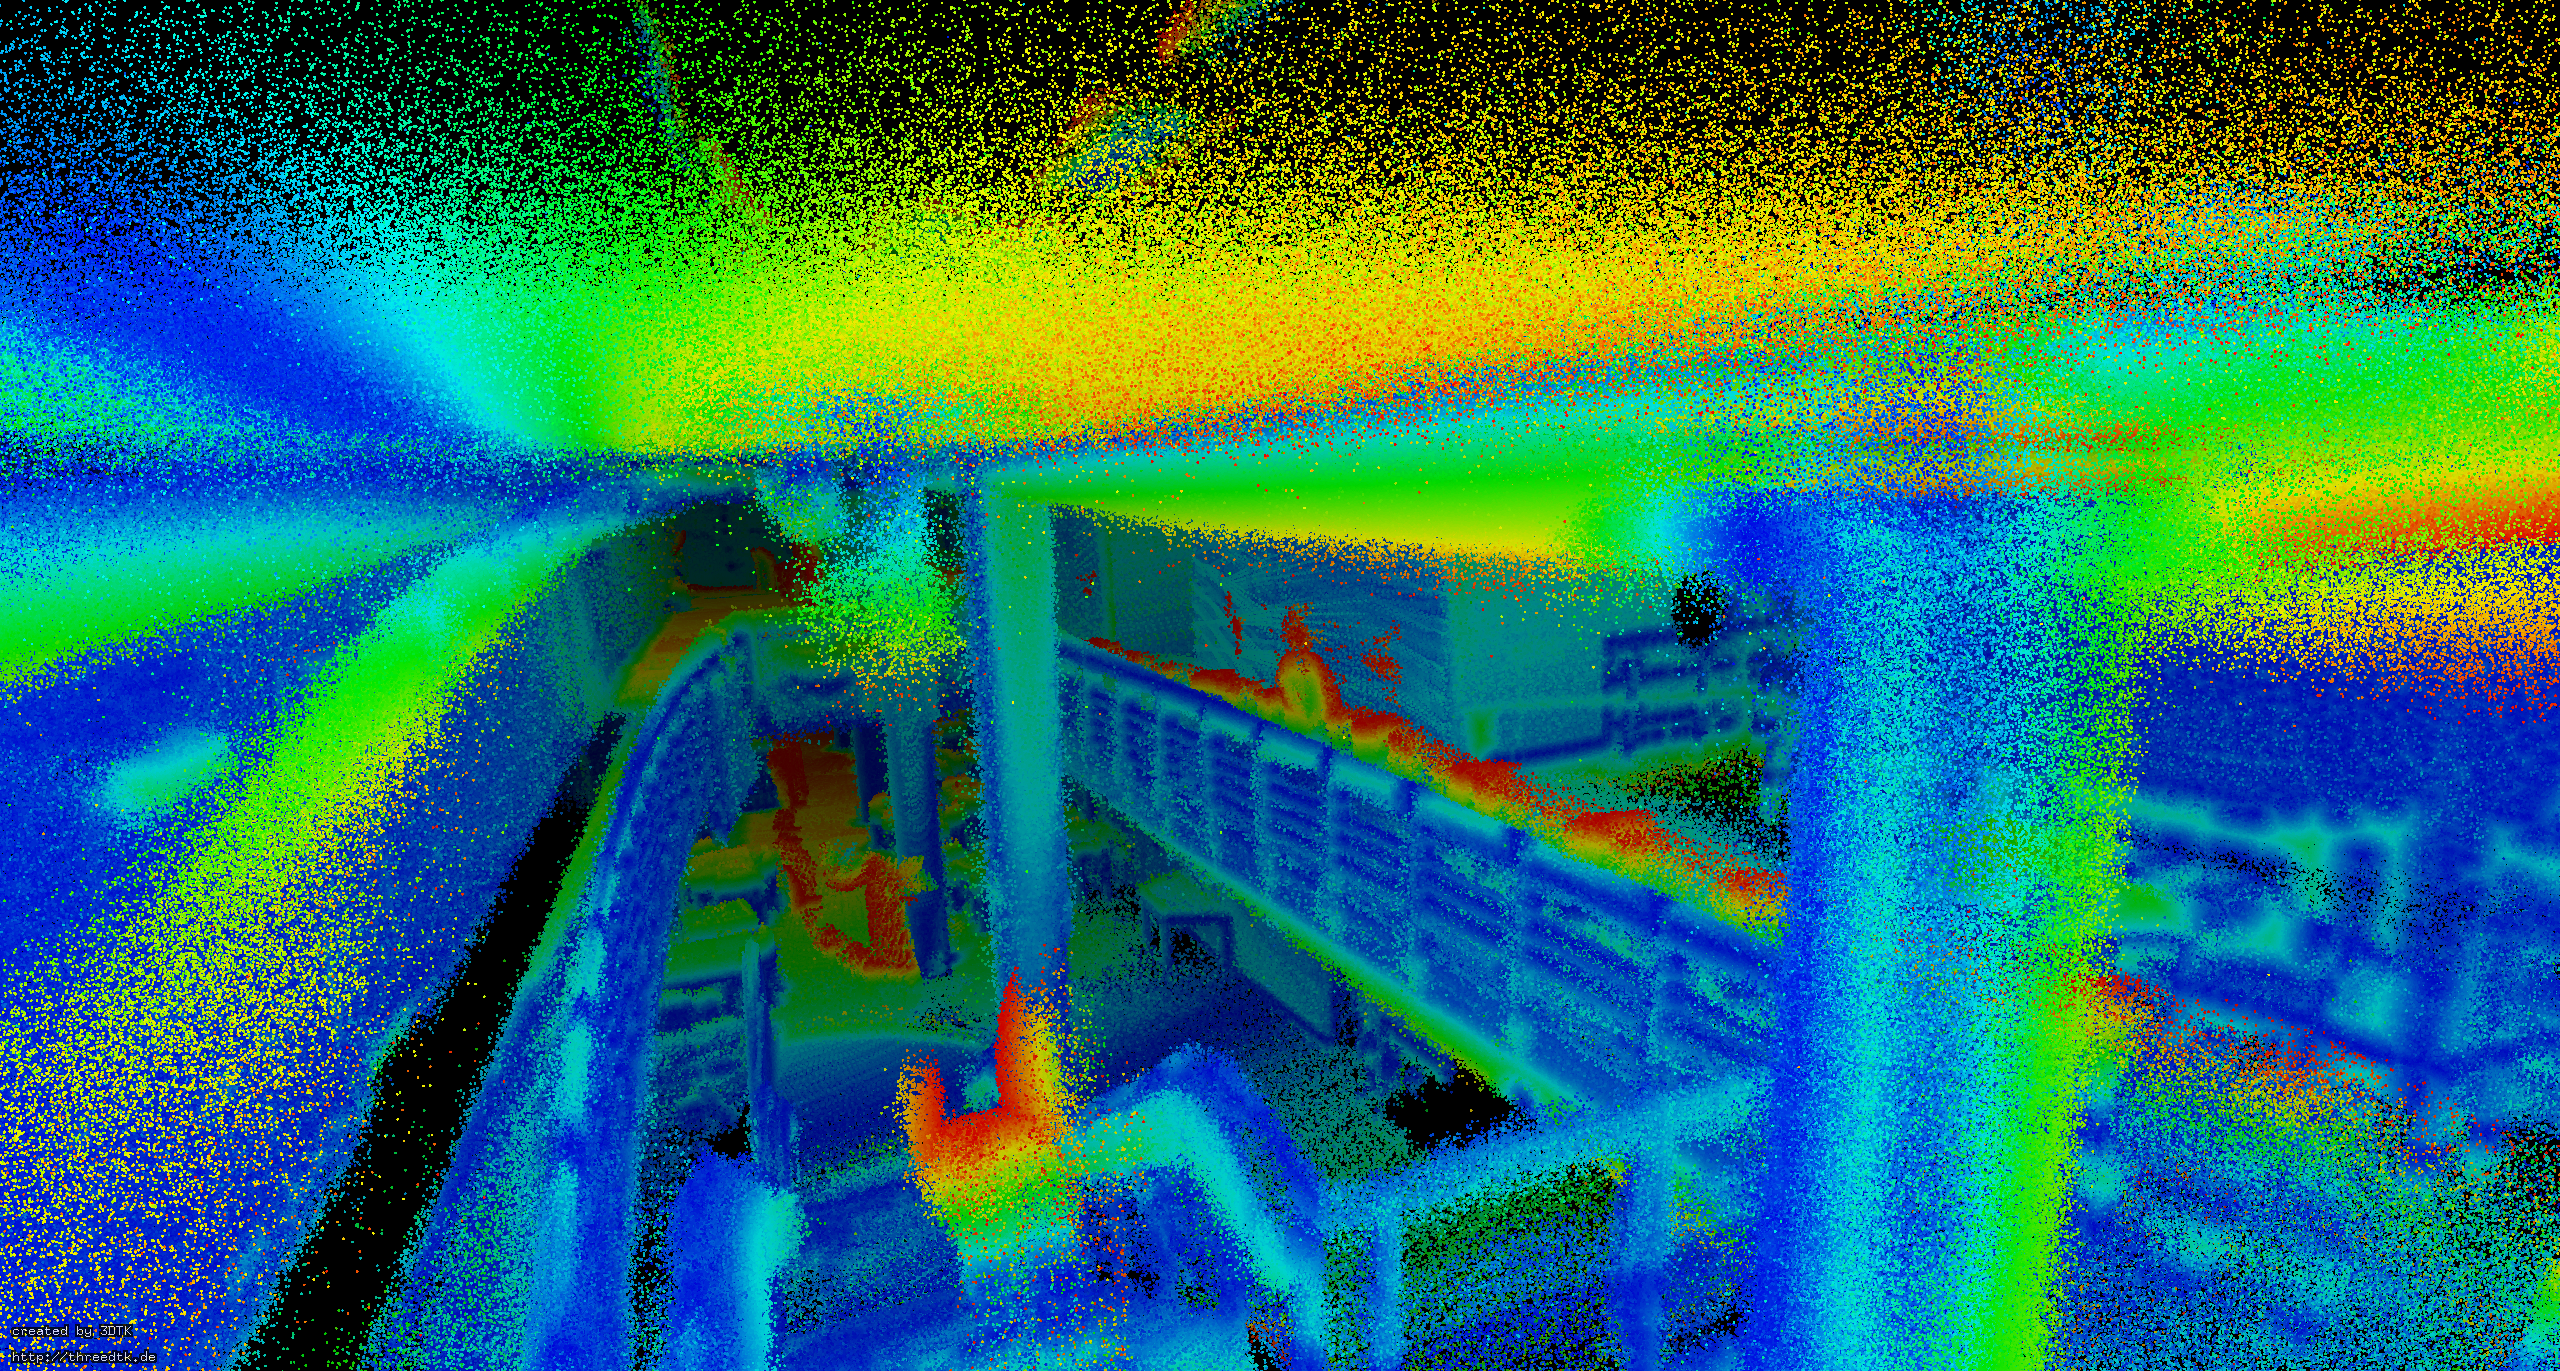
\includegraphics[width=\textwidth]{pics/results_images/a_dlio.png}
    \label{fig:results_act_dlio}
\end{subfigure}
\begin{subfigure}{0.195\textwidth}
    \centering
    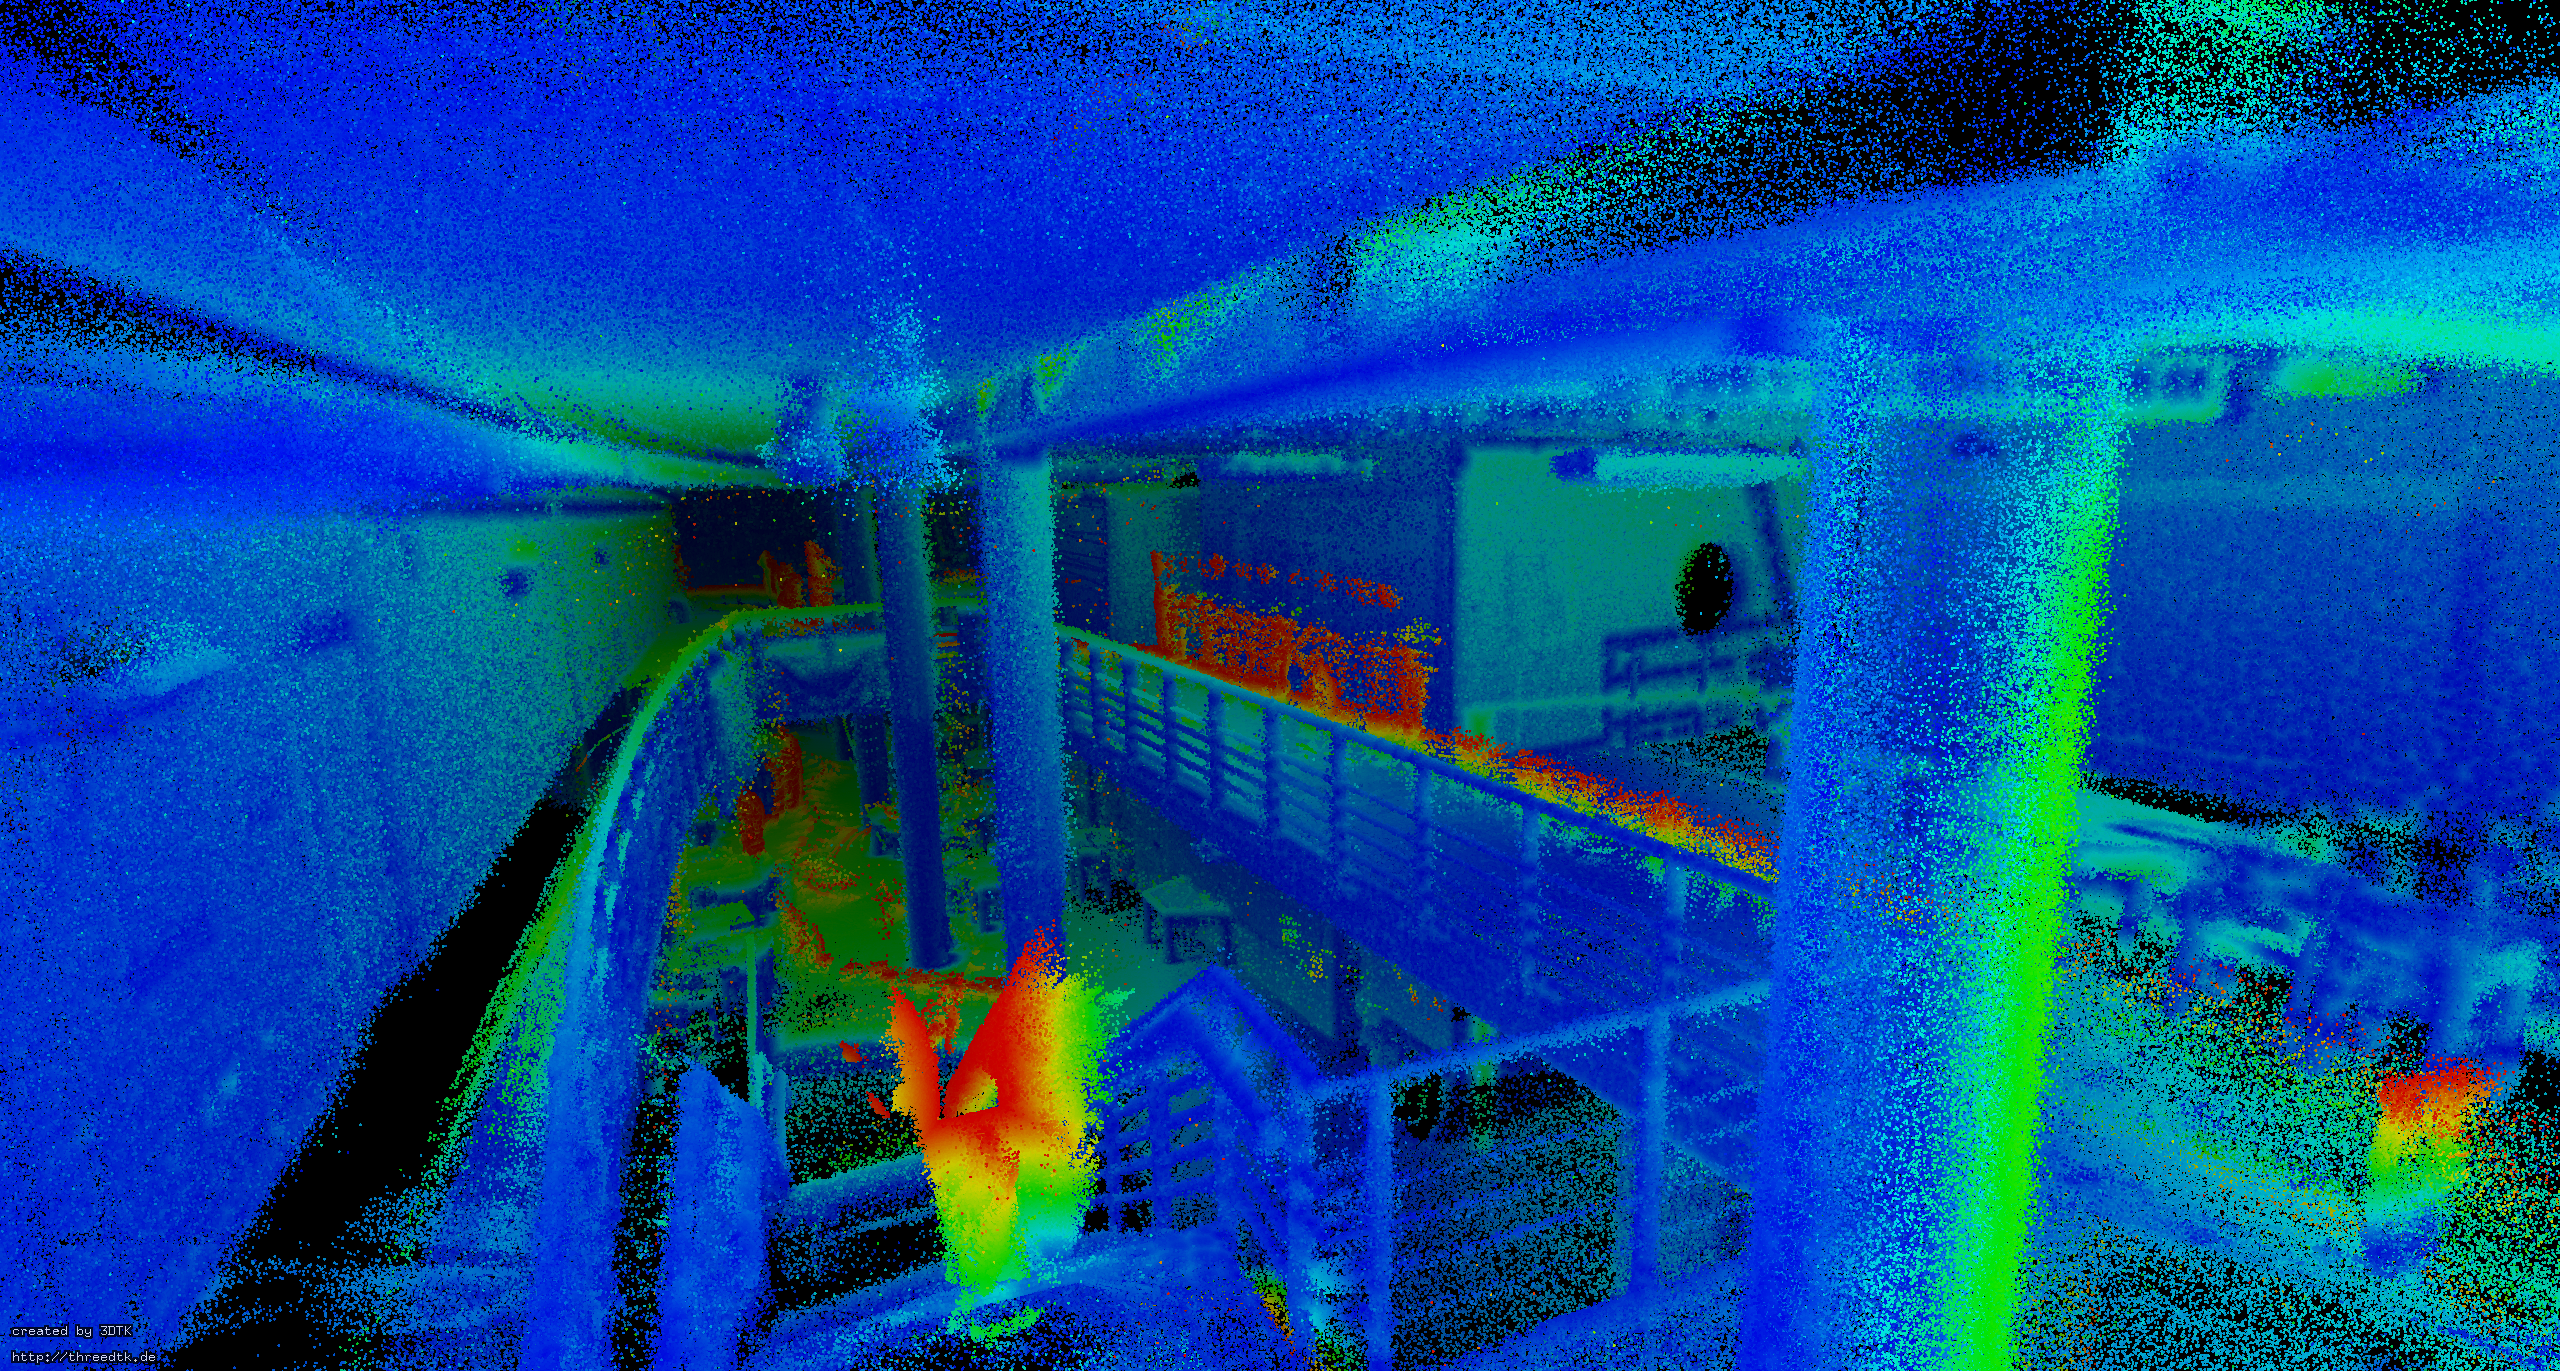
\includegraphics[width=\textwidth]{pics/results_images/a_livo.png}
    \label{fig:results_act_livo}
\end{subfigure}

% Second row - 2 subfigures (centered)
\begin{subfigure}{0.18\textwidth}
    \centering
    \includegraphics[width=\textwidth]{pics/histogram_results/histogram_cond_non_actuated_lio.png}
    \caption{Non-Act. Fast-LIO2}
    \label{fig:hist_non_lio}
\end{subfigure}
\hfill
\begin{subfigure}{0.18\textwidth}
    \centering
    \includegraphics[width=\textwidth]{pics/histogram_results/histogram_cond_non_actuated_livo.png}
    \caption{Non-Act. Fast-LIVO2}
    \label{fig:hist_non_livo}
\end{subfigure}
\hfill
\begin{subfigure}{0.18\textwidth}
    \centering
    \includegraphics[width=\textwidth]{pics/histogram_results/histogram_cond_actuated_lio.png}
    \caption{Act. Fast-LIO2}
    \label{fig:hist_act_lio}
\end{subfigure}
\hfill
\begin{subfigure}{0.18\textwidth}
    \centering
    \includegraphics[width=\textwidth]{pics/histogram_results/histogram_cond_actuated_dlio.png}
    \caption{Act. DLIO}
    \label{fig:hist_act_dlio}
\end{subfigure}
\hfill
\begin{subfigure}{0.18\textwidth}
    \centering
    \includegraphics[width=\textwidth]{pics/histogram_results/histogram_cond_actuated_livo.png}
    \caption{Act. Fast-LIVO2}
    \label{fig:hist_act_livo}
\end{subfigure}
\begin{subfigure}{0.16\textwidth}
    \centering
    \includegraphics[width=\textwidth]{pics/histogram_results/hsv.png}
    \caption{Color Mapping}
    \label{fig:hsv}
\end{subfigure}
\caption{Point Cloud Results and Error Distribution Analysis. A fly through video of the point clouds can be found at \url{https://youtu.be/1b0d2g3k4e8}. The first row shows the point clouds generated by comparing RIEGL map with each algorithm, while the second row displays the corresponding error distribution histograms.}
\label{fig:combined_results}
\end{figure*}

\section*{Conclusion and Future Work}
In this paper, we presented the design and evaluation of two spherical robots for 3D mapping applications. 
The first prototype, a \SI{16}{\centi\meter} diameter non-actuated sphere, demonstrated effective mapping performance using state-of-the-art LiDAR-inertial odometry algorithms on a compact and lightweight platform. 
The second prototype, a \SI{20}{\centi\meter} diameter actuated sphere, introduced a pendulum-based locomotion mechanism, enabling controlled movement and stabilization in addition to mapping capabilities. 
Both systems were evaluated in a controlled indoor environment. 
The non-actuated sphere using Fast-LIO2 achieved the lowest mean error and RMSE among all configurations. 
The actuated sphere showed strong potential for enhanced mobility and stability, marking a step forward in enabling more autonomous behaviors. 
These results highlight the feasibility and promise of spherical robots for 3D mapping and real-time SLAM on resource-constrained platforms such as the Raspberry Pi 5.
%Only limited algorithmic configurations were explored in this work. 
In future work, we plan to further optimize SLAM algorithm parameters specifically for spherical platforms, explore alternative actuation mechanisms, and evaluate performance in more dynamic and complex environments. 
The actuated sphere, in particular, can be developed further for autonomous navigation and exploration tasks, leveraging its enhanced locomotion capabilities. 
Additionally, integrating higher-resolution LiDAR sensors—such as the Robosense Airy—could improve mapping quality without increasing sphere's form factor. 
Pose estimation and the analysis of its associated errors were not addressed in this paper, as establishing accurate ground truth trajectories would require a separate measurement setup, which was beyond the scope of this study.
Overall, this work contributes to the growing field of spherical robotics and provides a foundation for future advancements in autonomous 3D mapping and mobile perception.
\bibliographystyle{IEEEtran}
\bibliography{bibliography}

\vspace{12pt}

\end{document}
